\xchapter{Systematic Literature Review}{  }
%Revisão sistemática de literatura}

\section{How a Systematic Literature Review works}

A Systematic Literature Review is an article selection method, which consists of the planning phase, review conducting and the analysis of the materials obtained. That kind of review uses a  protocol to formalize the search of bibliographical materials and aims to summarize empirical evidence, identify existing gaps in the researches carried out up to now and provide subsidies for new researches \citeonline{Kitchenham:2007}.

The planning phase consists in choose which topic will be studied, defines the research question which should be answered after articles analysis, select the keywords for the creation of the search string that will be used in databases, and are chosen by researcher the inclusion and exclusion criteria; in the conduct phase the search strings created should be applied in databases chosen in the previous phase; and in the last phase, a study of acquired materials is realized~\citeonline{Kitchenham:2007}. 

The choice of inclusion and exclusion criteria that will be applied in the article, should conform  following rule: if an article falls into at least one exclusion criterion, it must be refused, even if it fits into some criterion of inclusion, for an article to belong to the set of accepted articles must satisfy all inclusion criteria and none exclusion criteria~\citeonline{Kitchenham:2007}.

\section{Planning Phase}

The proposed systematic literature in this work aims to investigate what metrics and methodologies were applied to \ac{HHCRSP} until October 2017. so the following research question was defined:

\begin{itemize}
\item \emph{What metrics and methodologies have been used for \ac{HHCRSP} from 1998 to October 2017?}
\end{itemize}

In order to answer the question, we consulted articles of researchers that applied metrics and methodologies to \ac{HHCRSP}, having as one of the expected results the relation of the metrics and methodologies used in the period of time defined in the previous question.

The search for related articles was done with the following keywords:

\begin{itemize}
\item ``home health care''
\item ``home care''
\item nurse
\item routing
\item scheduling
\end{itemize}

Structured in the following search expression:

\begin{itemize}
\item \textit{``(``home health care'' OR ``home care'' OR nurse) AND routing AND scheduling''}
\end{itemize}

After the elaboration of the search expression, the inclusion and exclusion criteria were defined as a following.

\textbf{Inclusion criteria}
\begin{itemize}
\item Articles related to Home Health Care Routing and Scheduling Problem;
\item Articles published in journals or conferences;
\item Complete articles.
\end{itemize}

\textbf{Exclusion criteria}
\begin{itemize}
\item Articles published in languages that differ from English or Portuguese;
\item Inaccessible or unavailable articles;
\item Duplicate articles;
\item Articles published before 1998.
\end{itemize}

\section{Search conduct}

After defining inclusion and exclusion criteria of bibliographical materials, the following research bases were chosen, due to their popularity:

\begin{itemize}
\item Science Direct;
\item Springer;
\item Scopus;
\item IEEE Xplore;
\item ACM Digital Library.
\end{itemize}

After searches, 158 results were returned as organized in Figure:~\ref{bases}

\begin{figure}[H]
\begin{center}
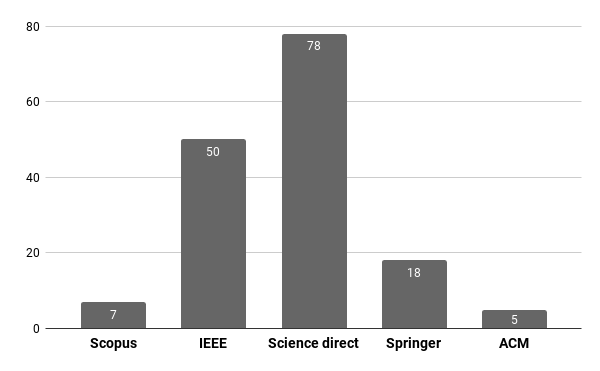
\includegraphics[width=0.4\textwidth]{base_de_dados_de_origem.png}
\caption{Counting by search bases \label{bases}}
\end{center}
\end{figure}

At the end of article selection, 19 articles were accepted because they attend all inclusion criteria and 139 articles were rejected because they don't attend at least one exclusion criterion or because they didn't attend some inclusion criteria. It is interesting to note that collected articles were published between 1998 and 2016, with a considerable increase in publications between 2012 and 2016, according to Figure~\ref{ano}.

\begin{figure}[H]
\begin{center}
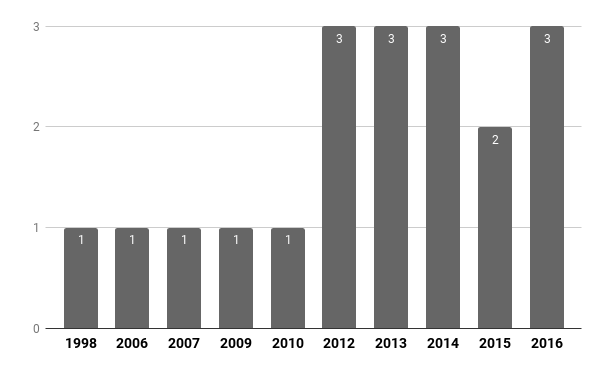
\includegraphics[width=0.4\textwidth]{contagem_por_ano.png}
\caption{Article Count by Publication Year \label{ano}}
\end{center}
\end{figure}

After applying the inclusion and exclusion criteria in the bibliographic materials, it was observed that 86.7\% of the articles were rejected. We believed that the reason for this high rejection rate was due to the relationship of the subject studied with existing publications in several health areas, causing the research bases to point to articles that later would not fit into any inclusion criterion.

\section{Related Literature Review}

To the best of our knowledge not exists other Systematic Literature Review about metrics and methodologies applied to \ac{HHCRSP}, it is believed that the lack of systematic literature reviews is because it is a problem that began to be explored at approximately 43 years. However, it finds some literature reviews published in 2017 by \citeonline{fikar:2017} and \citeonline{mohamed:2017}, but none of them fit the definition given by \citeonline{Kitchenham:2007} of systematic literature review, once the authors didn't elaborate an execution protocol to formalize the review and research process.

Although \citeonline{fikar:2017} have described the keywords used in their research, but their literature review hasn't a description of inclusion and exclusion criteria of the material searched nor define the databases where the material was collected. The review published by \citeonline{mohamed:2017}  described the search strings used and defined the databases where they did the research, but didn't create inclusion and exclusion criteria to define which materials suited his research.

The review of literature written by \citeonline{fikar:2017} aims compare different objectives, constraints and highlight future research in the \ac{HHCRSP} for which the author compared articles publishing between 1974 and 2016, from the following keywords: ``home care'', ``home health care'', ``routing'' and ``scheduling''.
The literature review developed by \citeonline{mohamed:2017} aims  analyze the existing literature on the \ac{HHCRSP}, for which the author compared materials of different natures, such as: scientific articles, book chapters, technical reports, thesis and dissertations published between 1997 and 2015 with following keywords: `home health care'', ``home care'' ``resource  scheduling'',  ``Routing'' and ``Vehicle Routing problem".

From results obtained in that review, it was established by \citeonline{fikar:2017} that \ac{HHCRSP} was first studied in 1974 from the article "A Model for Community Nursing in a Rural County", published by \citeonline{fernandez:1974}. 
Some articles found by \citeonline{fikar:2017} are directly related to \ac{VRPTW}, skills requirements and working time. 
They also verified the following solution techniques applied to the PERE: Variable Neighborhood Search, Branch and price, Fuzzy Simulated Evolution Algorithm, Genetic Algorithm, Memetic Algorithm, Multi-Directional Local Search, Particle Swarm Optimization, Repeated Matching, Simulated Annealing, Scatter Search and Tabu Search.

Was classified by \citeonline{mohamed:2017} constraints of patient, organization, professionals, such as temporal and geographical association. 

For patients, temporal constraints determine the frequency of visits,  time window of care and temporal dependencies; membership constraints determine preferences; geographical constraints determine the route between the residences.

For the organization, temporal constraints involve planning time and frequency of decisions; the restrictions of association guarantee continuity of care until the end of treatment; geographical constraints determine the service area. 

For professionals, the temporal restrictions have the utility of determining the hours worked; the restrictions of association are determined from the abilities of each nurse, temporal constraints determine the workplaces.

\section{Description of accepted Articles}

In that section, is described as accepted articles according to metrics and methodologies.

Motivated by Turkey reality of Home Care companies  \citeonline{tozlu:2016} developed the first approach of the Crew Constraints Home Care Routing Problem with Time Window, with the objective reducing the distance traveled by nurses in a day's work. To solve the problem was determined by  \citeonline{tozlu:2016}, a model of \ac{LIP} with the following objective function:

\begin{center}
$Min \sum D_{ij}x_{ij}$
\end{center}

Where $x_{ij}$ is a decision variable indicating that there is a path between $i$ and $j$.

The team was divided by \citeonline{tozlu:2016} into two groups: a group of nurses and a group of caregivers. Patients were divided into three groups: patients who needed nurses, patients who needed caregivers, and patients who needed both.
The vehicles used are identified as type 1, type 2 and type 3.
The objective of the problem is to determine the route traveled and the type of vehicle that each patient must attend in order to minimize the distance covered.

To determine the initial solution, the Variable Neighborhood Search was used by \citeonline{tozlu:2016} from the routes taken from \citeonline{Solomon:1987}, disregarding the capacity of the vehicle.
The tests were performed by \citeonline{tozlu:2016} from 192 instances based on the routes elaborated by Solomon for \ac{VRPTW} with 25 patients, finding good results for solutions with 175 instances within the time limit of two hours for the execution of each instance.

To determine the initial solution was used by \citeonline{tozlu:2016} the Variable Neighborhood Search with from the routes taken from \citeonline{Solomon:1987}, disregarding the capacity of the vehicle.
The tests were performed from 192 instances based on the routes elaborated by Solomon for \ac{VRPTW} with $25$ patients, finding good results for solutions with $175$ instances within the time limit of two hours for the execution of each instance.

Was proposed by \citeonline{trabelsi:2012} a mathematical model for \ac{HHCRSP} based on \ac{LIP} with the objective of minimizing discrepancy of the care worker workload, from the minimization the difference between the upper and lower limit of workload.
To solve the computational model, randomly obtained instances ranging from 4 to 15 patients and 2 to 4 nurses were used.

A case study was carried out by \citeonline{cattafi:2012} in a hospital in Ferrara, Italy, aiming at minimizing the maximum working hours and minimizing the number of different nurses visiting the same patient.

The constraint programming model for the \ac{HHCRSP} described by \citeonline{cattafi:2012} was formalized with the assistance of hospital's nursing team and consists of a finite set of services, being that for each service the patient is known, the day and the duration of the service, a finite set of nurses, a distance matrix and the travel time between the residences of two patients, the number of days considered in the scheduling, and the number of minutes available per day for each nurse.
In the model developed by the authors, each service is associated with a nurse, and a valid solution is one that respects all restrictions. The quality of the solution depends on the balance of the nurses' workload and how many different nurses care for the same patient.

The computational tests were performed with 15 nurses, who attend to 3323 requisitions of 458 patients in one month of work, each request having a duration ranging from 5 to 60 minutes. As a result, the authors concluded that the Logic Programming technique is an economically accessible technology to improve working conditions and quality of services.

Was proposed by \citeonline{trautsamwieser:2014} a solution to \ac{HHCRSP}, based on Branch and Price and Cut, in order to find the best route for the nurses and minimize the total work.
In case study realized at a hospital in Austria, \citeonline{trautsamwieser:2014} selected the care workers at levels: the care workers with a lower level are a charge of providing patient support services such as bathing or assisting in household tasks, the care workers with higher level provides medical, nursing services, and administer medications.

The computing tests \citeonline{trautsamwieser:2014} was elaborated with instances based on more than nine care workers, 45 clients and 203 visits during the week and instances based on 12 nurses, 60 clients, 255 visits, obtained from a data in Austria. Good results were obtained in the period of 1 hour, finding a viable solution.


Was carried out a case study by \citeonline{nguyen:2016} in a Home Care company in Lugano, Switzerland, aiming at solving allocation, routing and scheduling problems within a one week period.
In his paper, \citeonline{nguyen:2016} introduced an integrated model, based on genetic algorithms for the \ac{HHCRSP}, in which realistic characteristics as uncertainty in care workers availability, restrictions of time and work are taken into account.

To solve the problem, \citeonline{nguyen:2016} treated four optimization issues: rostering, assignment, routing and scheduling sequentially and iteratively.
The experiments were conducted from instances with 190 patients requiring 760 medical requirements from 15 nurses.

As results were observed by \citeonline{nguyen:2016}, that proposed algorithm works best with the strategy of replacing solutions at random, it is efficient for solution of large instances and provides a reliable solution against the uncertainty in the availability of nurses for the weekly planning and can be a tool to evaluate the tradeoff between robustness and  operational cost of a solution.

A heuristic goal based on swarms of fuzzy particles was used by \citeonline{mutingi:2013}, aiming at minimizing the imbalance of care workers working hours, for which the mean value of the working time of all care workers was calculated.

To perform the computational experiments \citeonline{mutingi:2013} used an illustrative example, drawn from \citeonline{bachouch:2010}, using instances with up to 15 nurses, but no in-depth discussion of the results was presented.

Was carried out by \citeonline {luna:2013} a case study on a multinational company, belonging to the group EULEN, that offers Home Care services.
Their study aimed to minimize the total daily workload of the caregivers and the number of caregivers who provide at least one service.

To address the problem, \citeonline {luna:2013} developed a parallelized evolution algorithm, capable of solving instances with up to 32 nurses and more than 10,000 services provided, however, the authors do not present a study of the optimality of the solutions obtained.

Was conducted by \citeonline{bachouch:2010} a study based on a French Home Care company with the aim of minimizing the discrepancy between care workers workloads. 
For this, was developed a solution based on \ac{LIP}  with the objective of balancing the workload among health professionals, as shown below:

Let $P_{max}$ and $P_{min}$ the upper bound and lower bound of working hours to the care workers. The workload balance is defined by \citeonline{bachouch:2010} as:  

\begin{center}
$Min~P_{max} - P_{min}$
\end{center}

To perform the computational experiment \citeonline{bachouch:2010}  used a randomly generated data with the maximum of five nurses, resulting in optimal schedules that provide tasks with a computation time of a few minutes or seconds.

The professionals of \ac{HHCRSP} were classified by \citeonline{Decerle:2016} between licensed and unlicensed. Licensed professionals offer medical services, such as drug administration and nursing services and unlicensed professionals offer home support services, such as help with household chores and personal hygiene.

Was as developed by \citeonline{Decerle:2016} a two-stage solution for \ac{HHCRSP} based on \ac{LIP},  aim to minimize costs related to moving and hours worked by licensed and unlicensed professionals.

Computational experiments were elaborated by \citeonline{Decerle:2016} from data obtained from two home care companies not identified by the authors. In these companies, nurses work from $6:45 \ am$ to $7:30 \ pm$, the visit time window is for a maximum of one hour. Licensed professionals have a cost of $50$ euros per hour and unlicensed professionals have the cost of $30$ euros per hour.

Were combined by \citeonline{Bertels:2006} solutions for \ac{HHCRSP} based on Constraint Programming, \ac{LIP}, and metaheuristics, aim to minimize transport costs and maximize patient satisfaction and care workers.

The metrics to define satisfaction of patients were defined by \citeonline{Bertels:2006} as follows:

\begin{itemize}
\item Choose the best time window to receive the service;
\item Choose the group of care workers you want to be treated;
\item Always be attended by the same care worker.
\end{itemize}

and satisfaction of care workers: 

\begin{itemize}
\item Choose the day off;
\item Choose work weekends;
\item Change patient, if there is any difficulty related to a particular care.
\end{itemize}

To model the problem \citeonline{Bertels:2006} addressed the routing aspect taking into consideration that health care professionals go to the patient's home through different types of transport: bicycle, car or public transport. A time window can represent the time interval in which a job should be started or describe the interval of time a nurse works.

For the computational tests, \citeonline{Bertels:2006} used 10 synthetic instances containing between 20 and 50 nurses and between 111 and 326 tasks, with the window of time between 6 and 72 minutes in random locations. The results were obtained in a maximum of 232 seconds, with the use of instances with 50 nurses, 200 patients, 600 services, from the results obtained, the authors concluded that the best results were generated by combining the efficacy of the \ac{LIP} to find the ideal starting points of jobs and the effectiveness of Constraint Programming to generate feasible ordering.

It was elaborate by \citeonline{Bierwirth:2013} a \ac{LIP} solution, with aim of minimizing the delay in patient care and maximizing customer satisfaction for the daily planning of \ac{HHCRSP}. 

To model the problem, \citeonline{Bierwirth:2013} differentiated the \ac{HHCRSP} services between single and double.
A single service consists of a service being run by a single team member while a dual service consists of at least one activity or service operation that is performed by two team members.
The double services were divided into simultaneous services and services with a certain precedence relation.
A concurrent service occurs when there is a need for more than one nurse to perform a particular service. For example, raising a person with a disability requires two members of a team.
Services with precedence relationships occur when the order of performance of services is important, i.e. the administration of medications prior to the provision of a meal.

Computational tests were generated by \citeonline{Bierwirth:2013} from seven sets of random instances, containing in each set, from 10 to 300 patients randomly located in a square area of 100x100 without taking into consideration the unit of measure and of 3 to 40 nurses, considering 6 types of services, with a time window of 120 minutes. With the time limit to 10 hours to run each instance.
As results, it could be observed that small instances returned optimum results in 20 seconds, whereas instances with more than 25 patients and 5 nurses failed to achieve good results within the established time, requiring the use of more powerful heuristics.

Was proposed by \citeonline{tricoire:2016} a mathematical model, based on \ac{LIP} with aim of maximizing patient satisfaction and minimizing the Home Care team traveled distance considering the team qualification and work laws.
For the computational tests, \citeonline{tricoire:2016} divided the instances into two sets. The first set contains 30 small sized instances with 20 to 25 services and the second set consists of real instances containing between 50 and 300 services. For each instance, the maximum and minimum work hours of the nurses were defined between 8 and 10 hours or between 4 and 6 hours respectively, providing six types of services.
The distance traveled study was generated from the OpenStreetMap tool and divided into four types of instances, taking into consideration the means of transportation used by the nurses (car or public transport) and the computational experiments were performed within two days. \cite{tricoire:2016} also found good solutions for small-sized instances, and it is necessary to construct meta-heuristics to construct an efficient solution for real instances.

The \ac{HHCRSP} was associated from \citeonline{Kergosien:2009} to Multiple Traveling Salesman Problem with Time Window and job restrictions whose some professionals can't attend simultaneously and some services need more than one professional simultaneously.

Looking for good solutions to \ac{HHCRSP} was elaborated by \citeonline{Kergosien:2009} a \ac{LIP} model with the aim to minimize the total route cost following by Home Care Workers. To realize the computational tests was used random instances with 1 to 3 skills and 20 to 40 services during between 10 minutes to 1 hour, with time window between 30 minutes to 3 hours tested with and without column generation technique and Euclidean distances in an area of 100x100.
After computational tests, \citeonline{Kergosien:2009} concluded that the proposed model isn't able to deal with real instances without column generation  

\citeonline{cheng:98} elaborated a \ac{LIP} model that aim minimize the home care worker overtime and a constructive greed heuristics.
The computational tests were realized by random instances with  40 and 20 hours home care workers with 10 patients and 30, 229 and 294 home care workers and 96 to 900 patients.

A \ac{LIP} metaheuristic was elaborated by \citeonline{calvo:2013} aim to minimize the travel distance following by home care workers and distributing the nurses' workload fairly.
To treat \ac{HHCRSP}, the authors divided the problem into two sets: In the first set, was used the edge coloring technique and in the second set was used the bin-packing method.

To do the computational tests, \citeonline{calvo:2013} used at least 190 instances proposed by \citeonline{Kergosien:2009}, composed of 30 services provided by 7 to 9 home care workers with 3 different skills.

To aim minimize the delay, cancellation and maximize the home care workers preferences, was realized a case study by \citeonline{rasmussenm:2012} with the Danish government where visits  between two and four hours, the home care workers have different working hours, are responsible for the own means of transportation with which they will go to patient's home and the visits have a precedence relation.
To solve the problem \citeonline{rasmussenm:2012} elaborated an exact branch-and-price algorithm and developed a modeling by \ac{HHCRSP} with \ac{LIP}.

The computational experiments elaborated by \citeonline{rasmussenm:2012} were carried out with four real instances provided by two Danish municipalities and complemented with 60 synthetic instances. Three quality parameters were measured: uncovered visits, home care preferences and total travel costs.

A study case was realized next to UK government by \citeonline{drake:2007} aim to optimize the working schedule to home care team who was handmade. To solve the problem,\citeonline{drake:2007} applied the particle swarm optimization.

\citeonline{drake:2007} made two computational experiments with real instances who contain 9 customers who receive care of nurses and caregivers in one week.
The first experiment analyzes the performance of presented technique with different parameter configurations in different instances of problems using the design of experiments Taguchi, a type of experiment that when managing control factors minimize noise, in which the authors used as control factor distances traveled and minimize the size of the team and maximize customer satisfaction.
The second experiment comparing solutions obtained manually by the UK government with solutions obtained by the authors.

A case study was realized by \citeonline{goos:2015} in a Home Care company in Belgium, belonging to \textit{Landelijke Thuiszorg} organization, aim to minimize the distance traveled by Home Care Workers and maximize two customers satisfy.

To obtain a solution to \ac{HHCRSP} was formulated by \citeonline{goos:2015} a \ac{LIP} model, the computational tests were realized with real instances contains 478 patients and 115 Home Care Workers obtained at home care company where the case study was realized.
According to \citeonline{goos:2015} from the solutions generated, the proposed model is able to for implementation in the specific case of the organization \textit{Landelijke Thuiszorg}.

Was elaborated by \citeonline{urli:2014}, Constraint Programming technique, a Branch-and-Bound and the Large Neighborhood search heuristic to solve the HHCRSP with the objective of minimizing the cost of travel by Home Care Workers.

The model presented by \citeonline{urli:2014} has two stages: In the first stage, is considered a single day and is assumed that all activities exactly require a caregiver, in the second stage more caregivers are added.

\citeonline{urli:2014} perform the computational tests with 18 groups with 30 instances each were randomly generated, totaling 540 instances, at a site of 40 $Km^{2}$, located in the center of Udine, Italy, differentiated by the planning horizon. 
From the results studied, the authors concluded that the Large Neighborhood search overcomes Restriction Programming when it comes to unassigned activities, on the other hand, the Restriction Programming technique is superior to Large Neighborhood search when it comes to reducing the total distance of displacement.